\chapter{Secrets of the nature}

    In this chapter, we will try to understand the world surrounding us thanks to a mathematical framework which describes the matter and its interaction.
    We will first have a look on the law that lead our Universe. Then, we will focus on the mathematical framework with the description of three interactions: the electromagnetism, the weak and the strong interactions.
    After that, we will study the electroweak interaction and the spontaneous symmetry breaking. We will finally discuss the limits of the theory and the solutions to avoid the limits. 
 \minitoc
  \section{The Standard Model}

    \subsection{Introduction}
    
    %\lettrine{\textgoth{T}}{he} 
    The Standard Model (SM) is a theory that describes the fundamental structure of the matter surrounding us. 
    It is one of the most successful achievement in modern physics.
    The elegant theoretical framework of the SM is able to provide good explanation of experimental results, but is also able to predict a wide variety of phenomena.

    The SM depicts the interactions between the fundamental constituents of matter, called particles.
    From a quantum point of view, a particle is defined by its intrinsic angular momentum, called spin. 
    That quantum number is a key to distinguish between the particle of 'matter' and the 'carrier force' particle.
    
    The half integers spin particles are obeying to the Fermi-Dirac statistics and are submitted to the Pauli exclusion principle:
    They can not occupied the same quantum state at the same time.
    These particles are called fermions.
    They are the constituents of the matter and are to the number of twelve.

    The fermions are divided into two categories: the leptons and the quarks. 
    The leptons are to the number of six: three charged particles and three neutral particles called neutrino.
    The first fundamental particle discovered in particle physics was the electron (e$^-$) at the end of the $19^{th}$ century.
    The two other charged leptons were discovered in 1937 for the muon ($\mu$) and in 1975 for the tau ($\tau$):
    Three neutrinos are associated to the three flavored leptons: the electron neutrino ($\nu_e$) discovered in 1953, the muon neutrino ($\nu_{\mu}$) in 1962 and the tau neutrino ($\nu_{\tau}$) discovered in 2000.

    The quarks are to the number of six.
    They can't be find alone in the nature.
    They are carrying a quantum number: the color.
    The color quantum numbers are green, blue and red (and the anti-color associated).
    They are always in a bounded state to form composite particles that are colorless and are called hadrons.
    A quark and an anti-quark form an integer spin composite particle, called meson.
    Three quarks bounded together are called baryons. The most known baryons are the proton and the neutron.
    They are made of the up quark (u) and the down quark (d).
    The other quarks were discovered in the second half of the 20$^{th}$ century.
    The strange quark (s) was discovered in 1968, followed by the charm quark (c) in 1974.
    Then, the bottom quark or beauty quark (b) was discovered in 1977.
    The last quark discovered was the top quark (t) in 1995.  

    The fermions are also divided into three categories that depends on the mass of the particle.
    The categories are called generations.
    The first generation of particles is composed of the electron, the electron neutrino, the u and d quarks. 
    They form the ordinary matter.
    The two other generations are particle that can be found in cosmic rays or in collision with accelerators.
    All the fermions and their properties is summarised in the table \ref{tab:fermions}.

    \begin{table}[!h]
      \begin{center}
        \begin{tabular}{c c c c c c c}
        \hline %----------------------------
        Type & Family & Particle  & L & B & Q$_e$ & Mass (MeV)  \tabularnewline
        \hline %----------------------------
        \hline %----------------------------
        \multirow{6}*{Leptons} & \multirow{2}*{1$^{st}$}    & $e$       & 1 & 0 & -1    & 0.511 \tabularnewline
                               & & $\nu_e$   & 1 & 0 & 0     & $< 2 \times 10^{-6}$ \tabularnewline
                               & \multirow{2}*{2$^{nd}$}    & $\mu$     & 1 & 0 & -1    & 105.66 \tabularnewline
                               & & $\nu_{\mu}$ & 1 & 0 & 0   & $< 2 \times 10^{-6}$ \tabularnewline
                               & \multirow{2}*{3$^{rd}$}    & $\tau$   & 1 & 0 & -1     & $1.78 \times 10^{3}$ \tabularnewline
                               & & $\nu_{\tau}$ & 1 & 0 & 0  & $< 2 \times 10^{-6}$ \tabularnewline
        \hline %----------------------------
        \hline %----------------------------
        \multirow{6}*{Quarks} & \multirow{2}*{1$^{st}$} & u & 0 & 1 & 2/3 & $2.3^{+0.7}_{-0.5}$\tabularnewline
                              & & d & 0 & 1 & -1/3 & $4.8^{+0.5}_{-0.3}$\tabularnewline
                              & \multirow{2}*{2$^{nd}$} & s & 0 & 1 & -1/3 & $ 95\pm 5 $ \tabularnewline
    		                  & & c & 0 & 1 &  2/3 & $1.275 \times 10^{3} \pm 2.5$ \tabularnewline
                              &\multirow{2}*{3$^{rd}$} & b & 0 & 1 & -1/3 & $4.66 \times 10^{3} \pm 30 $ \tabularnewline
        					  & & t & 0 & 1 & 2/3 & $ 173.21 \times 10^{3} \pm 511 \pm 711$\tabularnewline
        \hline %----------------------------        
        \end{tabular}
      \end{center}
        \caption{Summary of the 12 fermions. L is a quantum number associated to the leptons. Its value is 1 for leptons and -1 for anti-leptons. B is a quantum number associated to the baryons. It is equal to 1 for a baryon and to -1 for an anti-baryon. \cite{Agashe:2014kda} }
        \label{tab:fermions}
    \end{table}

    The second kind of particles are integer spins particles and are labelled bosons or gauge bosons.
    They are following the Bose-Einstein statistics 
    It means that the bosons are not limited to single occupancy of the same state as the fermions.
    The bosons are the mediator of the four fundamental interactions.    
    
    The electromagnetic interaction (EM) is mediated by the photon $\gamma$, a massless and chargeless particle of spin 1.
    The EM is responsible for the interaction between two charged particles.
    The weak interaction which is responsible of the $\beta$ radioactive decay (a nucleon is able to transform into an other one with the emission of a lepton and a neutrino).
    The gauge bosons bosons associated to the weak interaction are the neutral electrical charged boson $Z^0$, and two electrical charged one $W^+$ and $W^-$.
    The strong interaction is mediated by eight gauge bosons, the gluons.
    It is responsible for the nucleus cohesion and the hadrons.
    The last force is the gravitational interaction but it is not included into the SM.
    Trying to find a framework where the equation of the general relativity used to describe the macro world and the equation of the quantum mechanics describing the micro world is a difficult challenge.
    From a quantum theory, the boson associated to the gravitational force might be the graviton, a spin 2 particle. 

    The Higgs boson (H) is a particle predicted by the S.M and is the only one to have been found in 2012 at the LHC. 
    It is the gauge boson of the Higgs mechanism.
    This mechanism is the mass generator of particles and will be presented later REF TO LATER
    %assumed to be responsible for the generation of the masses and can be explained by the electroweak symmetry breaking.
    
    The table \ref{tab:bosons} summarises the different bosons of the SM.

  \begin{table}[!h]
    \begin{center}
        \begin{tabular}{c c c c c}
        \hline %----------------------------
        Force & Gauge bosons & Mass (GeV/$c^2$) & Electric charge & Range \tabularnewline
        \hline %----------------------------
        \hline %----------------------------
        Electromagnetic & $\gamma$ & 0 & 0 & $\infty$\tabularnewline  
        \multirow{2}*{Weak} & $Z^0$ & 91.1876 $\pm$ 0.0021& 0 & \multirow{2}*{$10^{-18}$ m} \tabularnewline
             & $W^{\pm}$ & 80.3980 $\pm$ 0.0250 & $\pm 1$  &\tabularnewline 
        Strong & g (8 gluons) & 0 & 0 & $10^{-15}$ m \tabularnewline
        \hline %----------------------------
        \hline %----------------------------
            & H & 125 GeV & 0 & \tabularnewline
        \hline %----------------------------
        \end{tabular}
    \end{center}
    \caption{Summary of the interactions and the boson defined by the Standard Model. \cite{Agashe:2014kda} \\ N.B.: the graviton was not included in this table because the gravitational force is not taken into account in the SM. }
    \label{tab:bosons}
  \end{table}
    
    \begin{figure}[h]
    \centering
      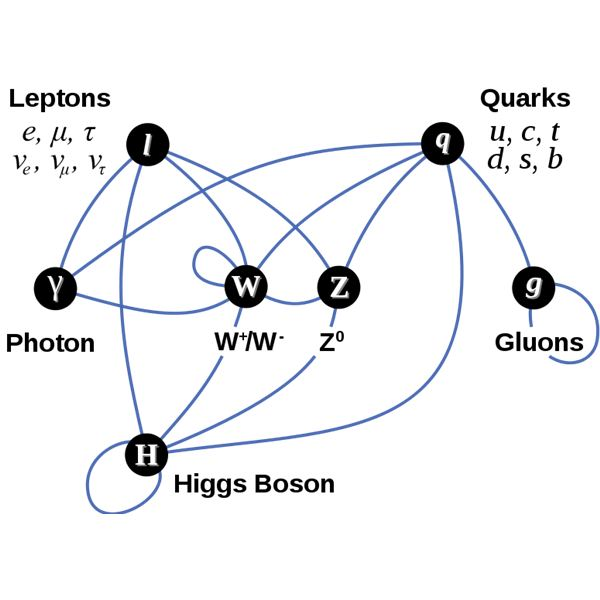
\includegraphics[width = 10cm]{Pictures/SM/elementaryParticles.jpg}
    %\missingfigure{Particles and boson}
    \caption{Summary of the Standard Model particles with their interactions.\\ \url{http://www.brighthub.com/science/space/articles/84750.aspx}}
    \label{fig:partInterac}
    \end{figure}
      
    \subsection{Quantum Field Theory}

	The mathematical basis of the SM is the Quantum Field Theory (QFT). All the interactions are described by the gauge group 
    
      \begin{equation}
    	SU_C(3) \otimes SU_L(2) \otimes U_Y(1)
	  \end{equation}
    
    The gauge theory is invariant under a continuous set of local transformation.
    Taking the gauge symmetries and the least action into account, physicists were able to set up equations that describe the dynamic of the interactions by Lagrangian.
    The steps to build Lagrangian for the three forces and the unification of the EM and weak interactions are going to be presented. 
    
      \subsubsection{Quantum Electrodynamic}

      The Quantum Electrodynamic (QED) is the QFT used to described the electromagnetic interactions using a $U(1)$ gauge group.
     The Quantum Electrodynamic (QED) is the QFT that combines the electromagnetism formalism and the quantum mechanics formalism to describe the interaction thanks to a relativistic Lagrangian.
     As the charge $Q_e$ of the electron is invariant on every part of the Universe, the QED Lagrangian should be invariant under some transformation.
     The $U(1)$ gauge group is a unitary group of one dimension that is invariant under space transformation.

      Lets first consider the Dirac equation for a free fermion:
      
      \begin{equation}
        \mathcal{L}_{Dirac} = \overline{\Psi}\left(x\right) \left(i \gamma^{\mu}\partial_{\mu} - m \right) \Psi\left(x\right)
      \end{equation}

      The Lagrangian is invariant under global U(1) transformation:

      \begin{equation}
            \begin{array}{rrccr}
             \Psi \left(x \right) & \rightarrow & \Psi^{'} \left(x \right)  & = & e^{-i\alpha} \Psi\left(x\right) \\
             \overline{\Psi}\left(x\right) & \rightarrow & \overline{\Psi}^{'}\left(x\right) & = & e^{i\alpha}  \overline{\Psi}\left(x\right) \\
            \end{array}
      \end{equation}

      The corresponding local symmetry is:

      \begin{equation}
            \begin{array}{rcccr}
             \Psi\left(x\right) & \rightarrow & \Psi^{'} \left(x \right) & = & e^{-i\alpha(x)} \Psi\left(x\right) \\
             \overline{\Psi}\left(x\right) & \rightarrow & \overline{\Psi}^{'}\left(x\right) & = & e^{i\alpha(x)}  \overline{\Psi}\left(x\right) \\
            \end{array}
      \end{equation}

      Considering the local symmetry, the mass term of the Lagrangian REF-Dirac-Lagrangian stays invariant but the term which contains the derivative is not anymore:
      By introducing a material derivative that includes a gauge field $A_{\mu}$, it is possible to keep the derivative invariant under local gauge transformation:

      \begin{equation}
        D_{\mu} \Psi\left(x\right) =  \left(\partial_{\mu} - i Q_e A_{\mu}\right) \Psi\left(x\right)
      \end{equation}

     The gauge field is not yet a dynamic field. To get a physical gauge field, a kinetic term should be added to the equation.
     This gauge invariant term that includes derivative from the $A_{\mu}$ field is:
    
     \begin{equation}
       F_{\mu \nu} \ = \ \partial_\mu A_\nu - \partial_\nu A_\mu
     \end{equation}

     The Lagrangian that is local invariant, is the one that describes the QED:

    \begin{equation}
    	\mathcal{L}_{QED} =  \overline{\Psi}\left(x\right)\left( i \gamma^\mu D_\mu - m \right) \Psi\left(x\right) - \frac{1}{4}F_{\mu \nu}\left(x\right) F^{\mu \nu}\left(x\right)
    \end{equation}

    A mass term $m A_{\mu} A^{\mu}$ for the field $A_{\mu}$ is missing because it is not gauge invariant. It can be explain by the fact that the photon is massless.

    \todo{Add details on the QED: coupling...}

    \subsubsection{Weak interaction}

    In 1930, Pauli assumed that the continuous energy spectrum of the electron in the $\beta$ decay could be explained by the existence of a new particle to respect the principle of energy conservation. 
    It is a light particle, that does not interact so much with matter.

    After the discovery of the neutron by Chadwick in 1932, Fermi wrote a theory on weak interaction to explain the $\beta$ decay. \cite{Fermi:1934hr} 
    He postulated that the neutron is decaying into a proton by emitting an electron and a light neutral particle, called neutrino.
    In analogy to the electromagnetism, he proposed a current-current Lagrangian to describe the $\beta$ decay.
    \begin{equation}
\mathcal{L}_{weak} = \frac{G_F}{\sqrt{2}}\left(\overline{p} \gamma_{\mu} n \right) \left(\overline{e} \gamma_{\mu} \nu \right)
    \end{equation}

    where the $G_F$ is the Fermi constant $G_F = 1.166 \dot 10^{-5} GeV^{-2}$. 
    
    Nevertheless, the non-relativistic limit leads to an incomplete theory.
    The interaction considered with a 2-components spinor transforms a proton to a neutron without changing the position, the spin or the parity.
    However, T.D. Lee and C.N. Yang have postulated in 1956 that the weak interactions violate the parity after analysing the decays of the $\tau$ and $\theta$ particles.\cite{1956PhRv..104..254L}
    The Wu experiment \cite{1957PhRv..105.1413W} confirmed that hypothesis in 1957 by studying the decay of $^{60}$Co.

    The Fermi interaction was modified by Feynman and Gell-Mann\cite{PhysRev.109.193} to a $V \ - \ A$ theory\footnote{$V$ stands for vector and $A$ stands for axial-vector}.
    The vector current are now subtracted by a axial vector current. For example, the neutrino current is replaced by:

    \begin{equation}
        \begin{array}{rrl}
        \overline{e}(x) \gamma_{\mu} \nu & \rightarrow & \overline{e}\gamma_{\mu}(1 - \gamma_5 ) \nu \\
            & & = \overline{e} \gamma_{\mu} \nu - \overline{e}\gamma_{\mu} \gamma_5 \nu \\
        \end{array}
    \end{equation}

    It was established that the weak current has the form $V \ - \ A$ instead of $V \ + \ A$.
    The weak interaction is only coupling left-handed particles and right-handed anti-particles.
    
    The lagrangian describing the weak interactions can be written as a currents interaction:

    \begin{equation}
      \mathcal{L}_{weak} = - \frac{G_F}{\sqrt{2}} J^{\mu}J_{\mu}^{\dagger}
    \end{equation}
    
     and $J^{\mu}$ is a combination of leptonic and hadronic current.

    Contrary to the QED, the weak interaction obeys to a non-Abelian symmetry group\footnote{A group is non-Abelian when the elements of the group do not commutate.}, the SU(2) symmetry group.
    The matter field could be represented as a doublet $\Psi_L$ and a singlet $\Psi_R$ of this group.

    \begin{equation}
      \begin{array}{cc}
        \Psi_L = 
         \begin{pmatrix}
           \nu_{eL} \\
           e_L
         \end{pmatrix}, & \Psi_R = e_R
      \end{array}
    \end{equation}

    The generators of the group are the three Pauli matrices $\sigma_i$, associated to a gauge field $W_{\mu}^a$.
    The bosons of the weak interactions are the $W^{\pm}$ and $Z$.

    As the left-handed leptons are combined into a doublet, a quantum number called weak isospin ($I_3$) is associated to them.
    The charged leptons has a weak isospin $I_3 = \frac{-1}{2}$ and for the neutrinos $I_3 = \frac{1}{2}$.
    Concerning the gauge bosons $W^{\pm}$ and $Z$, the weak isospin is respectively $I_3 = \pm 1, 0$.
    
    \subsubsection{Quantum Chromodynamics}
    
    The Quantum Chromodynamics (QCD) is the quantum field theory of the strong interaction.
    In this model, the interaction is due to a SU(3) gauge group. 
    It produces 8 gauge fields called gluons.
    The spinors of this theory are the six quarks that form a triplet with respect to the gauge symmetry.

    The SU(3) gauge group is a group of $9 - 1 = 8$ real parameters and of 8 generators. 
    Those generators are the Gell-Mann matrices. 
    The normalised generators are defined by: 
    
    \begin{equation}
        T^a = \frac{1}{2}\lambda^a
    \end{equation}

    The structure constant $f^{abc}$ can be expressed as:

    \begin{equation}
        if^{abc} = 2 Tr([T^a,T^b]T^c)
    \end{equation}
     
    Some theories arguments and the results of experiments in high energy physics ask to introduce six spinor fields, the quarks.
    Each of them are considered as a triplet state with respect to the SU(3) group:

    \begin{equation}
      q_i = 
        \begin{pmatrix}
          q_i^1 \\
          q_i^2 \\
          q_i^3 \\
        \end{pmatrix}
     \end{equation}
    
    where $q_i$ are the six quarks.
    These quarks can appeared in three different states, called color and that are named red, blue and green.

    The local gauge symmetry U(1) should be included into the SU(3) group.
    
    The gauge field $A_{\mu}$ can be introduced in the group:
    
    \begin{equation}
      A_{\mu} = g_S A^a_{\mu}\frac{\lambda^a}{2}
    \end{equation}
     
    with a = 1,...,8 and corresponds to the 8 gluons.
    A mass term  $m_g A^{\mu}_a A^a_{\mu}$ would not be gauge invariant, that implies the gluons are massless.

    The material derivative is then:

    \begin{equation}
      D_{\mu} = \partial_{\mu} - i A_{\mu} = \partial_{\mu} - i g_S A^a_{\mu} \frac{\lambda^a}{2}
    \end{equation}

    The QED field $F_{\mu \nu}$ is not gauge invariant in QCD.
    Nevertheless an additional term to obtain gauge invariant field tensor can be introduced:
    
    \begin{equation}
      G^a_{\mu \nu} = \left( \partial_{\mu} A^a_{\nu} - \partial_{\nu} A^a_{\mu} \right) + g_S f^{abc} A^b_{\mu} A^c_{\nu}
    \end{equation} 

    Finally, the QCD Lagrangian is given by:

    \begin{equation}
      \mathcal{L} = \sum_{i=1}^6  \bar{q_i} \left(i \gamma^{\mu}D_{\mu} -m_i \right)q_i - \frac{1}{4} G_{\mu \nu}^{a} G_{a}^{\mu \nu}
    \end{equation}
    

    \section{The Glashow-Weinberg-Salam model}

    Late 1960, a model of unification was postulated by Glashow, Weinberg and Salam\todo{Reference to the paper} to describe the electroweak interaction.
    It uses a same gauge theory leads by a $SU(2)_L \otimes U(1)_Y$ symmetry group, where the $SU(2)_L$ is the weak isospin group that was introduced in REF WEAK INTERACTION and $U(1)_Y$ is the weak hypercharge group.
    The weak hypercharge is related to the electric charge via Gell-Mann-Nishijima relation:
    \begin{equation}
      Q = I_3 + \frac{1}{2}Y
    \end{equation}

    The gauge field dynamic is given by the Lagrangian:

    \begin{equation}
        \mathcal{L}_{gauge} = - \frac{1}{2}W^a_{\mu\nu} W^{a\mu\nu} - \frac{1}{4}B_{\mu\nu}B^{\mu\nu}
    \end{equation}


    \begin{equation}
        \mathcal{L}_{GWS} = \mathcal{L}_{gauge} + \mathcal{L}_{leptons} + \mathcal{L}_{quarks}
    \end{equation}
    The quarks and leptons are 
    
    
    The Standard Model constitutes one of the most successful achievement in modern physics.
    One of its strength is to provides a elegant theoretical framework to describe the known experimental facts about particles, but also it was able to predict 
    the existence of a mechanism to generate the particle masses via the Higgs mechanism.

    With the lagrangians described above, the gauge boson were considered as massless fields.
    The electroweak interaction does not allow a $m\overline{\Psi}\Psi$ term because it does not transform as a scalar under $SU(2_L)\otimes U(1)g$.
    The $m^2A_{\mu} A^{\mu}$ violates the gauge invariance of the Lagrangian.
    That section will present the mechanism to generate fermions and boson masses.

  \begin{equation}
    \mathcal{L}_{E.W.} = i \overline{f} \partial_{\mu} \gamma^{\mu}f - g \overline{f}_L \gamma^{\mu} I_a W^a_{\mu} f_L - \frac{g'}{2}Y \overline{f} \gamma^{\mu} B_{\mu} f
    - \frac{1}{4} W^a_{\mu \nu}W^{\mu \nu}_a - \frac{1}{4}B_{\mu \nu}B^{\mu \nu}
  \end{equation}  

    \subsection{Symmetry Breaking mechanism and Goldston theorem}
    
    Before to introduce the Higgs mechanism, we will study the spontaneous symmetry breaking for a global symmetry.
    This phenomenon is also seen in phase transitions or laser theory.

    Lets consider first the Lagrangian density of a complex scalar field $\phi$:

    \begin{equation}
      \mathcal{L} = \partial^{\mu}\phi^{*} \partial_{\mu}\phi - \mu^2\phi^{*}\phi - \lambda (\phi^{*}\phi)^2
    \end{equation}

    The first component of the Lagrangian density corresponds to the kinetic term of a complex scalar field.
    The second component is related to a scalar potential.

    The coefficient $\mu^2$ is a real parameter. Nevertheless, depending on its sign, the potential can take two forms.

    If $\mu^{2} > 0$, the symmetry is unbroken and the potential has a minimum at $\phi = 0$ that is not degenerate.

    When $\mu^{2} < 0$, the minima of the potential is located on a circle of radius: 

    \begin{equation}
      v = \sqrt{\frac{- \mu^2}{2\lambda}} > 0
      \label{eq:v}
    \end{equation}

    The symmetry is then spontaneously broken.

    Lets consider a new field $\phi$:

    \begin{equation}
      \phi(x) = \frac{1}{\sqrt{2}} \left( v + \rho(x) + i\Phi(x) \right)
    \end{equation}

    The value $v$ is given by one of the solution from equation \ref{eq:v}, $h(x)$ and $\Phi(x)$ are real fields.

    The Lagrangian density is then given by:

    \begin{equation}
      \mathcal{L} = \frac{1}{2} (\partial_{\mu}\rho)^2 + \frac{1}{2}(\partial_{\mu}\Phi)^2 - \lambda v^2 \rho^2 - \lambda v (\rho^3 +\rho \Phi^2) - \frac{\lambda}{4}(\rho^2 + \Phi^2)^2
    \end{equation}

    The field $\rho(x)$ is a massive field coupled to the massless field $\Phi(x)$.
    Its mass is $m_{\rho} = 2 \mu^2$.

    The field $\Phi(x)$ corresponds to the massless bosons called Goldstone bosons.


    \subsection{Higgs mechanism}

    As we have seen with the Lagrangian of the QED and QCD, the bosons generated are massless. Nevertheless, the W$^{\pm}$ and the Z bosons have a mass. 
    The origin of the fermions masses is solved in the SM thanks to the Higgs-Englert-Brout mechanism. \cite{PhysRevLett.13.508}

    Lets consider first a complex scalar doubled field $\Phi$:
    
    \begin{equation}
       \Phi = \begin{pmatrix}
                \phi^{+}\\
                \phi^{0}
              \end{pmatrix}
    \end{equation}

     The invariant Lagrangian density under $SU(2)_L \otimes U(1)_Y$ gauge transformation is:

    \begin{equation}
      \mathcal{L} = \left(D^{\mu} \phi \right)^{\dagger} \left( D_{\mu} \phi \right) - V(\phi)
      \label{eq:lagrangianHiggs}
    \end{equation}    
    
    The covariant derivative is given by:
    
    \begin{equation}
      D_{\mu} = \partial_{\mu} + i g \frac{\sigma^i}{2} W^i_{\mu} + i\frac{g'}{2}YB_{\mu}
    \end{equation}        
    
    As seen before, $\mu^2$ could be positive or negative.
    We will focus only on the negative case. 
    The minima of the field is obtained for these configuration: 

    \begin{equation}
      v = \sqrt{\frac{- \mu^2}{2\lambda}} > 0
      \label{eq:v}
    \end{equation}

    Lets expand the field $\Phi$ around its minima by including a field $h(x)$ that describes quantum fluctuations:

    \begin{equation}
      <\Phi_0> = \begin{pmatrix}
                   0 \\
                   v + h(x)
                 \end{pmatrix}
      \label{eq:fieldHiggs}
    \end{equation}

    The substitution of \ref{eq:fieldHiggs} into \ref{eq:lagrangianHiggs}, 

%    The first term corresponds to the kinetic term of a scalar field.
%    The second term is a scalar potential that is invariant under $SU(2)_L$ and it is:
%
%    \begin{equation}
%      \begin{array}{lr}
%        V(\phi) = \mu^{2}\phi^{\dagger}\phi + \lambda \left(\phi^{\dagger}\phi\right)^2  & , with \ \lambda > 0 \\
%      \end{array}   
%    \end{equation}
    
    
    Depending on the sign of $\mu^{2}$, the potential can take two forms.
    If $\mu^{2} > 0$, the potential has a minimum at $\phi = 0$ and describes a scalar particle with a mass $\mu$ and a quartic self coupling.
    As the transformation $\phi \rightarrow  - \phi$ is respected, this solution is a symmetric one.

    When $\mu^{2} < 0$, there is not a unique ground state for this system but multiple states with the same vacuum energy.
    
    the minima is obtained for those fields configurations:

    \begin{equation}
      v = \sqrt{\frac{- \mu^2}{2\lambda}} > 0
      \label{eq:v}
    \end{equation}

    This minima will be considered as a vacuum state.
    Lets write a new field:

    \begin{equation}
      \phi(x) = v + h(x) + i \Phi(x)
      \label{eq:fieldHiggs}
    \end{equation}

    The value $v$ is given by one of the solution from equation \ref{eq:v}, $h(x)$ and $\Phi(x)$ are real fields.
    The Lagrangian density becomes then: 

    \begin{equation}
    \begin{array}{rcl}
        \mathcal{L} & = & D^{\mu}h D_{\mu}h - \left[ \mu^2\left(v^2 + h^2 + 2vh\right) + \lambda \left(v^4 + 4v^3h + 6v^2h^2 + 4vh^3 + h^4\right)\right] \\
                    & = & D^{\mu}h D_{\mu}h - \left[ h \left( 2\mu^2v + 4\lambda v^3 \right) + h^2 \left(\mu^2 + 6 \lambda v^2 \right) + 4 \lambda v h^3 + \lambda h^4 + \left( \mu^2v^2 + \lambda v^4 \right) \right]
      \end{array}
    \end{equation}

    The second term is equal to zero, the third one to $-2 \mu^2$, and the last one is a constant and does not affect the physics, so we will not take it into account.
    Finally, it leads to the Lagrangian below:

    \begin{equation}
      \mathcal{L} = D^{\mu}hD_{\mu}h - \left( -2\mu^2h^2 +4vh^3 + \lambda h^4 \right) 
    \end{equation}
    
    In the case where $-\mu^2 < 0$, the Lagrangian describes a scalar field $h$ of mass $m_h^2 = -2 \mu^2$ and that his self interacting ($h^3$ and $h^4$ terms in the Lagrangian).

    \begin{figure}[h]
    \centering
      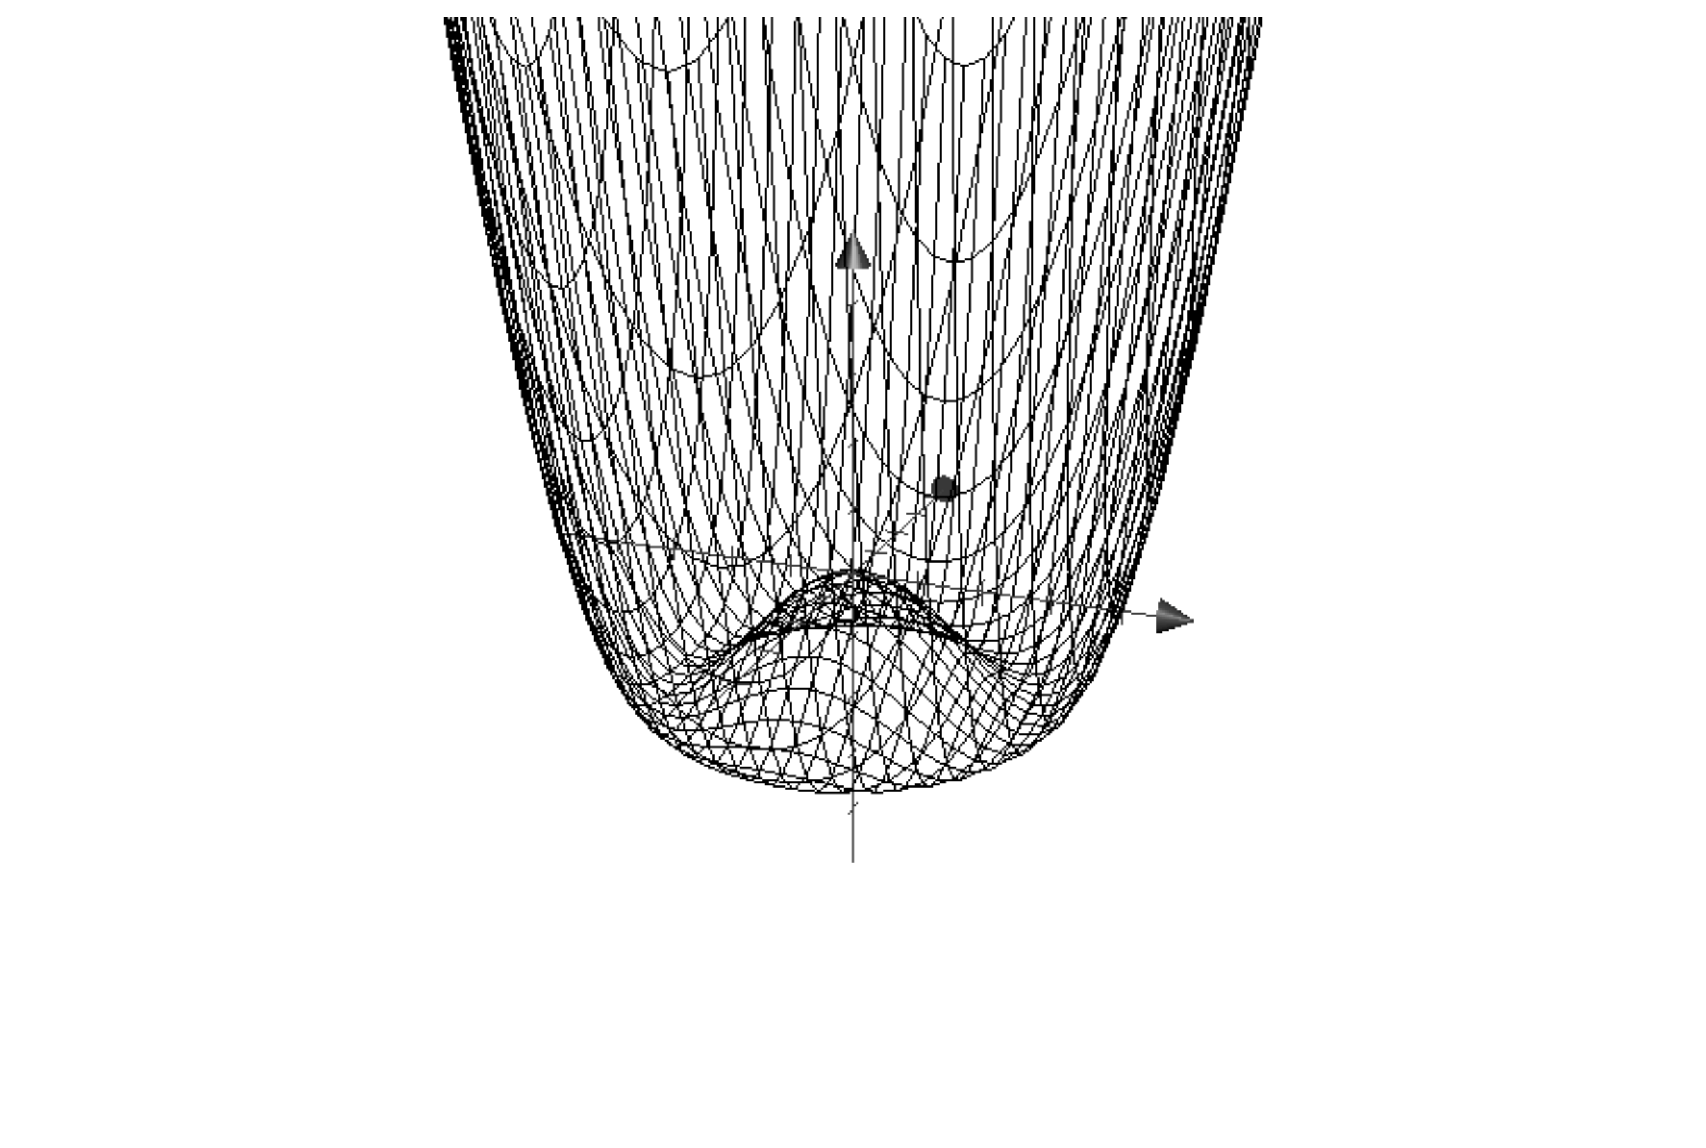
\includegraphics[width = 10cm]{Pictures/SM/mexHat.eps}
      %\missingfigure{Mexican hat}
    \caption{Scalar potential: ADD A GOOD CAPTION.}
    \label{fig:scalarPotential}
    \end{figure}

    Here talk about the Higgs mechanism but may be added in a Higgs chapter...


  % \subsubsection{Higgs Decays}

  % As explained before, the Higgs boson couples to all particles of the Standard Model.
  % The figure \ref{fig:higgsBR}, the branching ratios for different decay modes are shown as a function of the mass of the Higgs boson.
  % For a Higgs mass of 125.5 GeV, a large number of decays are accessible to experiments

  %  \begin{figure}[h]
  %  \centering
  %  \missingfigure{Higgs Branching ratio}
  %  \caption{The branching ratio of the Higgs}
  %  \label{fig:higgsBR}
  %  \end{figure}

  % \subsubsection{Higgs production at the ILC}
  %  
  %  \begin{figure}[h]
  %  \centering
  %  \missingfigure{Higgs Production}
  %  \caption{Higgs production}
  %  \label{fig:higgsBR}
  %  \end{figure}
      
  \section{Beyond the Standard Model}

  The SM is one of the best theory to describe the infinity and beyond. 
  Nevertheless, it can not explain all the mysteries in the universe. 
  This theory conforms experimental data in high energy physics but is unsatisfactory.
  
  \subsection{Limitations of the Standard Model}

  Despites the fact the experimental results are not contradictory to the SM, the theory is far away to be the answer to all the questions.
  The particle physics community is facing a challenge to find the ultimate theory of everything.
  A exhaustive lists of some limitations are going to be presented.

    \subsubsection{Free parameters}

    The SM does not explain the existence of the free parameters, which are to the number of 19.
    It does not explain also why there are three generations of particles and also why the gap between generations is spread over five orders of magnitude.

    This is not a problem for the physics, but the community has a lack to understand these values.
  
    \subsubsection{Hierarchy problem}

    The hierarchy problem refers to two main scales problem about the SM.

    First of all, the difference between the energy scale of the SM and the Planck scale is of the seventeen orders of magnitude.
    No "intermediate" physics have been found between the two scale.

    A second problem occurs while considering the Higgs boson mass.
    The SM does not predict its mass.
    However, 
    The theoretical Higgs mass is higher that what it should be compared to EW scale.

    This problem is known as the fine-tuning problem. 
    The Higgs interacts with the particles of the SM (fermions, W and Z boson), but it also interacts with himself.
    Due to the scalar nature of the boson, they are quartic divergences while calculating the loop corrections.
    
    \subsubsection{Gravitation}

    Although particles physicists are dreaming of a "theory of everything" that will unify the electroweak, strong and gravitational interactions,
    there is no viable theory to describe the gravity in a quantum point of view to include it in the SM and that will be still valid at a macro-scale.

    \subsubsection{Neutrino mass}

    The neutrinos defined buy the SM are assumed to be exactly massless.
    Nevertheless at the end of the 90's, the Super Kamiokande experiment had surprising results.
    There was a lack on the expected solar and atmosphere neutrino flux. 
    The results was interpreted by an oscillation of neutrinos between the three leptonic flavors.
    However, the oscillation is possible only if the neutrino has a mass.
    That phenomenon could be considered as a proof of physics beyond the SM.

    \subsubsection{Matter-antimatter asymmetry}

    As discussed at the beginning of this chapter, the SM defines equal number of particles and anti-particles. 
    Although everyone assumes that the matter and antimatter was created in exactly equal amount by the Big Bang, a mechanism has favoured electrons, protons and neutrons to positrons antiprotons and antineutrons.
    If the amount of matter and antimatter was equal, our Universe would have been completely annihilated.
    The matter domination could be a local phenomenon with an antimatter surrounding region. 
    However, the region of contact between matter and antimatter would be a violent place that should disturb the cosmic microwave background 

    An assumption to explain the asymmetry is that the antimatter was produced in an infinity proportion compared to the matter.
    Hence, the annihilation as lead to create a Universe only made of matter.
    A mechanism which tends to prefer the matter has been observed in the study of the kaon oscillation.
    This particle is able to transform spontaneously to its own anti-particle and vice-versa.
    Nevertheless, this transformation is not symmetric: the kaon is slower to turn into an anti-kaon than the inverse transformation.
    Unfortunately, the SM provides no explanation about that mechanism.
 
    \subsubsection{Dark Matter}
    
   % \todo{Rephrase dark matter and dark energy}
    Several astrophysical observations are indicating that the Universe is made not only of visible matter but also of matter that seems to be invisible to the electromagnetic interaction, the dark matter.
    It was found that the matter of the SM describes only 5\% of the Universe content. 
    The rest of the Universe is made of 22\% of dark matter and around 73\% of dark energy.
    The neutrinos are possible candidates to dark matter, as it couples to SM matter via only weak interaction, but they cannot account for the entire density of the universe.
    Nowadays only twelve particles (plus the anti-particles associated) have been observed. 
    The idea of dark matter comes from the way we estimate the mass of galaxy.

    \subsection{Theories beyond the Standard Model}

      \subsubsection{Supersymmetry}
    
      The Supersymmetry (SUSY) is a QFT, that relates the elementary fermions known to a corresponding boson and the bosons to a corresponding fermion.
      The related particles are called superpartners.
      They have the same mass, the same quantum numbers but the spin is differing by a $\frac{1}{2}$ factor.
      SUSY might be a broken symmetry. 
      This will allow the super-particles to acquire very high masses.

      SUSY is a good candidate for physics beyond the SM. 
      It will solves the hierarchy problem without any fine tuning.
      It will be able to provide a framework for the unification of the 3 gauges interaction at a GUT scale.
      The lightest superparticle is a good candidate for the Dark Matter.

      Despites it will answered many questions from the SM, there is a lack to understand why SUSY is a broken symmetry.
      
      \subsubsection{Grand unification theory}
      
      After the success of the electroweak unification, the next step is to include the strong interaction to build the Grand Unification Theory (GUT), an extension of the SM.
      In this framework, the three forces are different manifestations of a single interaction. 
      It includes the $SU(3)_C \otimes SU(2)_L \otimes U(1)_Y$ symmetry group into a larger $SU(5)$ group. 
      The quarks and leptons are ordered in left decuplets and right quintets.
      The coupling constants are described by only one parameter.  
      There are 24 mediators, the 12 mediators of the SM plus 6 X mediators (charge $\pm4/3$ and 3 colors) and 6 Y mediators (charge $\pm1/3$ and 3 colors).
      It predicts the existence of new particles as leptoquarks\footnote{Coupling between a lepton and a quark}, multiple Higgs bosons, new currents.

      Unfortunately, the theory is not validated because of its prediction of the proton life time. 
      The first GUT was introduced by Georgi and Glashow in 1974 and was predicting a decay of the proton. 
      The actual experimental limit of the proton life-time is set to $5 \times 10^{32}$ years, whereas the predicted life-time defined by the SU(5) group is one order of magnitude lower.
      \todo{Ref Review of particle physics}

      \subsubsection{Technicolor}

      The technicolor is a theory that explains the mass generation.
      Contrary to the EW symmetry, the masses of particles is not generated by the spontaneous symmetry breaking but it is generated by a strong gauge interaction.
      This interaction is strong and confined at the energy that have been experimentally probed.
      The approach of the theory avoids the hierarchy problem induced by the SM.
      
      \subsubsection{String theory}

      The particle physicists have the dream of unifying the forces of the nature to have only one single interaction with four different manifestations.
      The string theory proposes a framework for the "theory of everything".
      The basic unit of matter is no more considered as particles but one-dimensional string of which particles are various vibrational modes.

      The string theory is a theory of quantum gravity.
      It tries to unify the gravitation to the quantum 
      Extra dimensiosn of 10 -11 space time dimensions.
      Possible explanation for the hierarchy problem.

    \section{Conclusions}

    We have seen the beauty and the limits of the SM.
    The high energy physics community is trying to study as far as possible the limit of the SM and also try to find some proof of new physics beyond the SM.
    The Large Hadron Collider (LHC) at CERN has permitted in 2012 to point out the existence of a Higgs boson.  
    Nevertheless, the beam structure of the LHC is not efficient enough to perform very precise measurements.
    Because of the collision between protons, one does not know exactly the energy of the collision.
    We will discuss in the next chapter a future experiment where electrons and positrons are used to probe the matter instead of protons and antiprotons.
